\id{IRSTI 61.61.09}{https://doi.org/10.58805/kazutb.v.4.25-610}

\begin{articleheader}
\sectionwithauthors{K.B. Vernigorov, S.V. Nechipurenko, B.B. Yermukhambetova, V.V. Bushkov, G.S. Irmukhametova, A.Zh. Alikulov, O.V. Stoyanov, Y.M. Kazakov, S.A. Efremov}{INFLUENCE OF CARBONISED RICE HUSK FILLER ON CHANGES IN
DEFORMATION AND STRENGTH PROPERTIES OF POLYETHYLENE DURING THERMAL
AGEING}

{\bfseries \textsuperscript{1}K.B. Vernigorov, \textsuperscript{2,3}S.V.
Nechipurenko, \textsuperscript{2,3}B.B. Yermukhambetova,
\textsuperscript{4}V.V. Bushkov,}

{\bfseries \textsuperscript{2,3}G.S. Irmukhametova,
\textsuperscript{2,3}A.Zh. Alikulov\textsuperscript{\envelope },
\textsuperscript{5}O.V. Stoyanov, \textsuperscript{5}Y.M. Kazakov,
\textsuperscript{2,3}S.A. Efremov}
\end{articleheader}

\begin{affiliation}
\textsuperscript{1}SIBUR PolyLab LLC, Moscow, Russia,

\textsuperscript{2}Al-Farabi Kazakh National University, Almaty,
Kazakhstan,

\textsuperscript{3}National Engineering Academy of the Republic of
Kazakhstan, Almaty, Kazakhstan,

\textsuperscript{4}SIBUR LLC, Moscow, Russia,

\textsuperscript{5}Kazan National Research Technological University,
Kazan, Russia

\raggedright \textsuperscript{\envelope }Corresponding author: \href{mailto:alikulov.adilet@gmail.com}{\nolinkurl{alikulov.adilet@gmail.com}}
\end{affiliation}

The influence of a new filler of natural origin on the thermal oxidation
process of high-pressure polyeth-ylene has been studied. The studied
filler is carbonized rice husk, a waste product of agricultural
production. It has been established that CSF exhibits some
thermostabilising effect, preventing the decrease of deforma-tion and
strength characteristics of the~polymer after its exposure for 3 hours
at 170ºC. The introduction of CSF allows to keep the yield strength at
the level of 77\% (10\% wt. CSF) and 46\% (5\% wt. CSF), while for
unfilled aged LDPE this index does not exceed 3\% of the initial sample.
The breaking stress of the filled samples remains at the level of the
unoxidized ones. A synergetic effect was revealed when the investigated
filler and standard antioxidant Irganox 1010 were used. At
the~introduction of 10\% wt. of CSF and 0,2\% wt. of phenolic
stabilizer, there is no decrease in destructive stress after the~thermal
aging of the material.

{\bfseries Keywords:} polyethylene, filler, carbonized rice husk,
thermo-oxidation, strain-strength characteristics.

\begin{articleheader}
{\bfseries КӨМІРТЕКТІ КҮРІШ ҚАБЫҒЫНЫҢ ТОЛТЫРҒЫШЫНЫҢ ТЕРМИЯЛЫҚ ҚАРТАЮ
КЕЗІНДЕ ПОЛИЭТИЛЕННІҢ ДЕФОРМАЦИЯЛЫҚ БЕРІКТІК ҚАСИЕТТЕРІНІҢ ӨЗГЕРУІНЕ
ӘСЕРІ}

{\bfseries \textsuperscript{1}К.Б. Вернигоров, \textsuperscript{2,3}С.В.
Нечипуренко, \textsuperscript{2,3}Б.Б. Ермухамбетова,
\textsuperscript{4}В.В. Бушков, \textsuperscript{2,3}Г.С. Ирмухаметова,
\textsuperscript{2,3}А.Ж. Аликулов\textsuperscript{\envelope },
\textsuperscript{5}О.В. Стоянов, \textsuperscript{5}Ю.М. Казаков,
\textsuperscript{2,3}С.А. Ефремов}
\end{articleheader}

\begin{affiliation}
\textsuperscript{1}«СИБУР ПолиЛаб» ЖШС, Мәскеу, Ресей,

\textsuperscript{2}әл-Фараби атындағы Қазақ ұлттық университеті, Алматы,
Қазақстан,

\textsuperscript{3}Қазақстан Республикасының Ұлттық инженерлік
академиясы, Алматы, Қазақстан,

\textsuperscript{4}«СИБУР» ЖШС, Мәскеу, Ресей,

\textsuperscript{5}Қазан ұлттық технологиялық зерттеу университеті,
Қазан, Ресей,

е-mail: \href{mailto:alikulov.adilet@gmail.com}{\nolinkurl{alikulov.adilet@gmail.com}}
\end{affiliation}

Жаңа табиғи толтырғыштың жоғары қысымды полиэтиленнің термототығу
процесіне әсері зерттелді. Зерттелген толтырғыш -- бұл ауылшаруашылық
өндірісінің қалдықтары болып табылатын көміртекті күріш қабығы. ККТ
170ºС температурада 3 сағат бойы экспозициядан кейін полимердің
деформациялық-беріктік сипаттамаларының төмендеуіне жол бермейтін кейбір
термостабилизациялық әсер ететіні анықталды. ККТ енгізу аққыштық шегін
77\% (ККТ 10\% масс.) және 46\% (5\% масс. ККТ) деңгейінде сақтауға
мүмкіндік береді, бұл ретте толтырылмаған ескірген ЖҚПЭ үшін бұл
көрсеткіш бастапқы үлгі көрсеткіштерінің 3\%-дан аспайды. Толтырылған
үлгілердің деструктивті кернеуі тотықпаған деңгейде сақталады.
Зерттелген толтырғыш пен стандартты антиоксидант Ирганокс 1010-мен бірге
пайдалануда синергетикалық әсер анықталды. 10\% масс. ККТ және 0,2\%
масс. фенолды тұрақтандырғыш енгізгенде материалдың термиялық қартаюынан
кейін деструктивті кернеудің төмендеуі байқалмайды.

{\bfseries Түйін сөздер:} полиэтилен, толтырғыш, карбонизацияланған күріш
қабығы, термототығу, деформация және беріктік сипаттамалары.

\begin{articleheader}
{\bfseries ВЛИЯНИЕ НАПОЛНИТЕЛЯ ИЗ КАРБОНИЗОВАННОЙ РИСОВОЙ ШЕЛУХИ НА
ИЗМЕНЕНИЕ ДЕФОРМАЦИОННО-ПРОЧНОСТНЫХ СВОЙСТВ ПОЛИЭТИЛЕНА ПРИ ТЕРМИЧЕСКОМ
СТАРЕНИИ}

{\bfseries \textsuperscript{1}К.Б. Вернигоров, \textsuperscript{2,3}С.В.
Нечипуренко, \textsuperscript{2,3}Б.Б. Ермухамбетова,
\textsuperscript{4}В.В. Бушков, \textsuperscript{2,3}Г.С. Ирмухаметова,
\textsuperscript{2,3}А.Ж. Аликулов\textsuperscript{\envelope },
\textsuperscript{5}О.В. Стоянов, \textsuperscript{5}Ю.М. Казаков,
\textsuperscript{2,3}С.А. Ефремов}
\end{articleheader}

\begin{affiliation}
\textsuperscript{1}ООО «СИБУР ПолиЛаб», Москва, Россия,

\textsuperscript{2}Казахский национальный университет имени аль-Фараби,
Алматы, Казахстан,

\textsuperscript{3}Национальная инженерная академия Республики
Казахстан, Алматы, Казахстан,

\textsuperscript{4}ООО «СИБУР», Москва, Россия,

\textsuperscript{5}Казанский национальный исследовательский
технологический университет, Казань, Россия,

е-mail: \href{mailto:alikulov.adilet@gmail.com}{\nolinkurl{alikulov.adilet@gmail.com}}
\end{affiliation}

Изучено влияние нового наполнителя природного происхождения на процесс
термоокисления полиэтилена высокого давления. Исследованный наполнителя
представляет собой карбонизированную рисовую шелуху, являющуюся отходом
сельскохозяйственного производства. Установлено, что УКН проявляет
некоторое термостабилизирующее действие, препятствуя снижению
деформационно-прочностных характеристик полимера после его экспозиции в
течении 3-х часов при 170ºС. Введение УКН позволяет сохранить предел
текучести на уровне 77\% (10\% масс. УКН) и 46\% (5\% масс. УКН), в то
время для ненаполненного состаренного ПЭВД этот показатель не превышает
3\% от показателей исходного образца. Разрушающее напряжение наполненных
образцов сохраняется на уровне неокисленных. При совместном
использовании исследованного наполнителя и стандартного антиоксиданта
Ирганокс 1010 выявлен синергетический эффект. При введении 10\% масс.
УКН и 0,2\% масс. фенольного стабилизатора не наблюдается снижения
разрушающего напряжения после термического старения материала.

{\bfseries Ключевые слова}: полиэтилен, наполнитель, карбонизированная
рисовая шелуха, термоокисление, деформационно-прочностные
характеристики.

\begin{multicols}{2}
{\bfseries Introduction.} Polymer composite materials due to the complex of
their valuable qualities are widely used in many spheres of human
activity. The use of fillers of various types (dispersed, fibrous,
woven) allows not only to increase the strength characteristics of the
material, but also to change its thermal, electrical, frictional, and
other characteristics. The combination of thermoplastics, fillers of
different natures and aggregate states, stabilizers, plasticizers, and
other additives in the polymer composition allows to create materials
with the widest range of properties and meeting the requirements of the
most demanding areas of industry. However, during the processing of
polymers into products and their further operation as a result of
thermal-oxidative aging, the performance of the material deteriorates
and its service life is reduced. Therefore, one of the important objects
of research is the influence of various components of composite
material, in particular fillers, on the resistance of polymers to
various types of degradation.

A number of publications have been devoted to the study of thermal aging
processes of filled polymers, including polyethylene {[}1-4{]}. However,
they mainly consider the processes of aging and stabilization of
polymers filled with mineral fillers.

At present, carbon-silica composite is proposed as a filler from natural
renewable raw materials, which is carbonized rice stalk and husk waste
in a pyrolysis furnace without access to oxygen at a temperature of
550-600°C {[}5{]}. According to {[}6{]}, the composition of
carbon-silicon filler (CSF) includes 47,26 \% carbon, 50,38 \%
SiO\textsubscript{2}, and 2,36 \% impurities, mainly oxides of various
metals.

Since a number of researchers {[}7-10{]} note the presence of
a~synergetic effect of rubber hardening at the joint use of carbon black
and silicon dioxide, there is an increasing number of works on the study
of the influence of complex filler CSF on the properties of various
rubbers {[}11-15{]}.

The aim of the study was to investigate the influence of carbon-silica
filler obtained from natural raw materials on the thermal aging
processes of high-pressure polyethylene.

{\bfseries Materials and methods.} High-pressure polyethylene (LDPE) of
15313-003 grade (GOST 16337-77, changes 1-3) and carbon-silicon filler
provided by «NeoCarbon» LLP (Republic of Kazakhstan) were used as
objects of research. Characteristics of polyethylene are given in Table
1. The chemical composition of CSF filler is shown in Table 2.
Irganox-1010 (pentaerythrol
tetrakis(3-(3,5-di-tert-butyl4-hydroxyphenyl) propionate) produced by
BASF was used as a stabilizer.
\end{multicols}

\begin{table}[H]
\caption*{Table 1 -- Characteristics of polymers}
\centering
\begin{tabular}{|p{0.12\textwidth}|p{0.12\textwidth}|p{0.12\textwidth}|p{0.12\textwidth}|p{0.12\textwidth}|p{0.12\textwidth}|}
\hline
Polymer   & Melt flow rate, g/10 min, T=190ºС & Melting point, ºС        & Yield strength, MPa       & Tensile breaking stress, MPa & Relative elongation at break, \% \\ \hline
15313-003 & \multicolumn{1}{c|}{0,35}         & \multicolumn{1}{c|}{106} & \multicolumn{1}{c|}{10,8} & \multicolumn{1}{c|}{14}      & \multicolumn{1}{c|}{450}         \\ \hline
\end{tabular}
\end{table}

\begin{table}[H]
\caption*{Table 2- Chemical composition of carbon-silica filler}
\centering
\begin{tabular}{|l|c|}
\hline
\textbf{Chemical composition} & \multicolumn{1}{l|}{\textbf{Contents, \%}} \\ \hline
Carbon                        & 47,26                                      \\ \hline
SiO2                          & 50,38                                      \\ \hline
Na2O                          & 0,04                                       \\ \hline
MgO                           & 0,16                                       \\ \hline
Al2O3                         & 0,01                                       \\ \hline
P2O5                          & 0,11                                       \\ \hline
K2O                           & 1,72                                       \\ \hline
CaO                           & 0,28                                       \\ \hline
TiO2                          & 0,01                                       \\ \hline
MnO                           & 0,02                                       \\ \hline
Fe2O3                         & 0,01                                       \\ \hline
\end{tabular}
\end{table}

\begin{multicols}{2}
Polymer compositions were prepared by mixing in melt in a Brabender
mixer for 10 minutes after loading all components. The mixing
temperature was 150°C. Rotor speed150 rpm.

Samples for physical and mechanical tests were obtained by pressing
(GOST 12019-2021) at a temperature of 160°C. After pressing all samples
were subjected to conditioning at room temperature for a day (GOST
12423-2013).

Aging of the samples was carried out at 170ºC for 1, 2, and~3 h.

Determination of deformation and strength properties of the samples was
carried out on a tensile testing machine TestP 108 with automatic
registration of results at a speed of 500 mm/min in accordance with GOST
11262-2017.

{\bfseries Results and discussion.} Currently, there is a large amount of
information on the~successful modification of thermoplastics with
mineral fillers to improve their performance. The study of the
possibility of using inexpensive fillers of natural origin in
polyethylene-based compositions is of undoubted interest for the
development of new polymeric materials.

The investigations have shown that the introduction of the studied
filler practically does not affect the strength of the material, only
slightly reducing the breaking stress of the composition. The increase
in the concentration of CSF expectedly leads to a constant monotonic
deterioration of the elasticity of the material (Fig. 1). At the same
time, the relative elongation at break for LDPE filled with less than 4
\% wt of CSF remains at the same level as that observed in LDPE filled
with a similar amount of other dispersed fillers.
\end{multicols}

\begin{figure}[H]
	\centering
	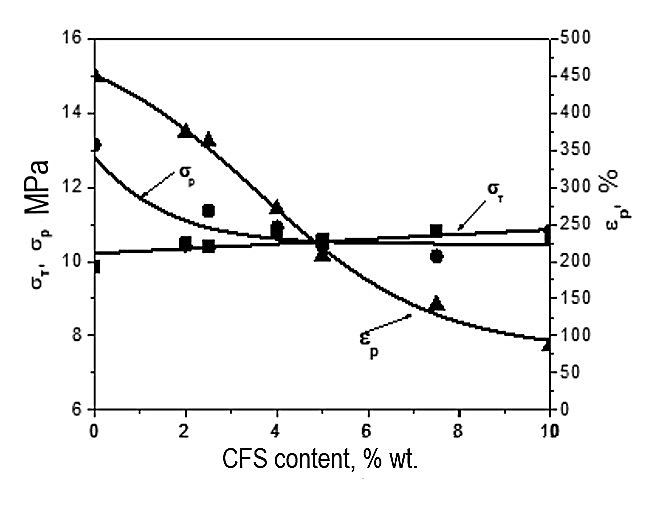
\includegraphics[width=0.4\textwidth]{media/chem/image19}
	\caption*{Fig. 1 -- Influence of CSF concentration on deformation and
strength characteristics of LDPE}
\end{figure}

\begin{figure}[H]
    \centering
    \begin{subfigure}[t]{0.4\textwidth} % Align at the top
        \centering
        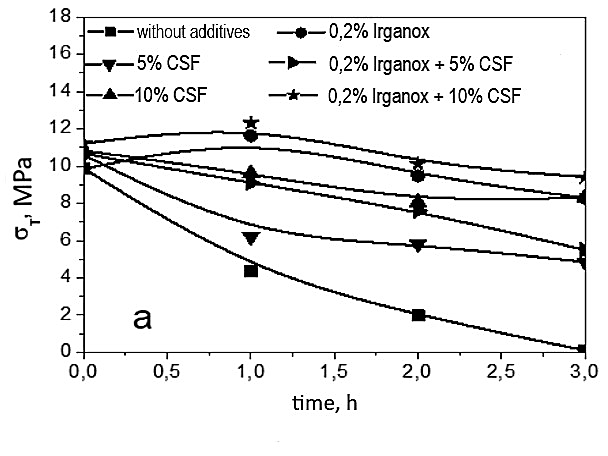
\includegraphics[width=\textwidth]{media/chem/image20}
    \end{subfigure}
    \hspace{0.05\textwidth} % Adjust horizontal space between the subfigures
    \begin{subfigure}[t]{0.4\textwidth} % Align at the top
        \centering
        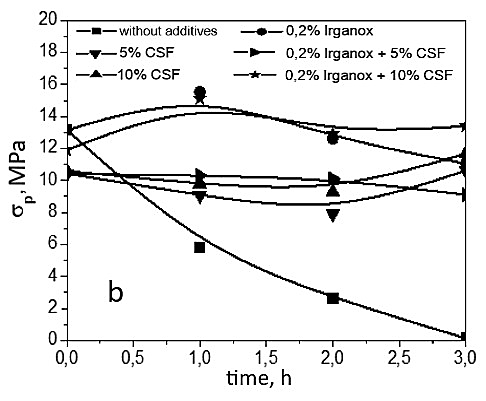
\includegraphics[width=\textwidth]{media/chem/image21}
    \end{subfigure}
    \caption*{Fig. 2 -- Change of yield strength (a) and breaking stress (b)
of composites in the process of thermal aging}
\end{figure}

\begin{multicols}{2}
Since in addition to carbon black and silicon oxide, the CSF contains
2.36 \% of impurities, which are oxides of various metals, it was of
interest to evaluate the effect of this filler on the thermo-aging
process of LDPE.

In the course of the research, it was found that the strength
characteristics of LDPE filled with carbonized rice husk during aging
decrease to a lesser extent than for unfilled polyethylene (Fig. 2, 3).
This indicates the manifestation of some stabilizing properties by this
filler. At the same time, the joint introduction of filler and CSF
allows to keep the level of strength characteristics for a longer time
(Fig. 3). Inhibition of the process of oxidation and destruction of
polyethylene at the~introduction of complex carbon-silicon filler is
probably connected with the presence of metal oxides, which are able to
interact with carboxyl groups formed at thermo-oxidation of polymer. The
use of the antioxidant Irganox 1010 in the composition of polyolefin
composition together with CSF preserves the strength properties of the
aged material at the level of the initial unaged composite. That~is
probably connected to some synergetic action of the filler and
antioxidant.
\end{multicols}

\begin{figure}[H]
    \centering
    \begin{subfigure}[t]{0.4\textwidth} % Align at the top
        \centering
        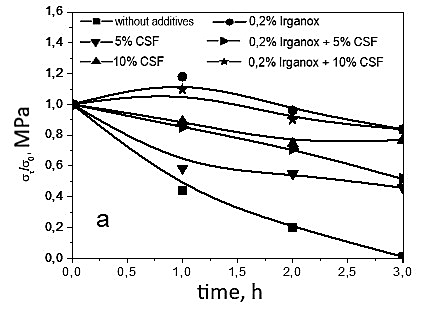
\includegraphics[width=\textwidth]{media/chem/image22}
    \end{subfigure}
    \hspace{0.05\textwidth} % Adjust horizontal space between the subfigures
    \begin{subfigure}[t]{0.4\textwidth} % Align at the top
        \centering
        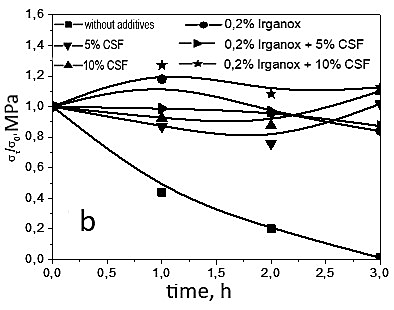
\includegraphics[width=\textwidth]{media/chem/image23}
    \end{subfigure}
    \caption*{Fig. 3 -- Rate of yield stress (a) and failure stress (b) of
composites in the process of thermal aging}
\end{figure}

\begin{multicols}{2}
Polyethylene filled with CSF has significantly worse elasticity than the
original one (Fig. 1), but in the process of its thermal aging the
decrease in relative elongation at break is much slower (Fig. 4).
Relative elongation of the samples aged for 3 hours at 170ºC, filled
with 5 and 10\% of CSF, is 65 and 40\% of the values of samples not
subjected to aging. The combination of UCS and the standard stabilizer
of phenolic type Irganox1010 almost completely stops the reduction of
elasticity of the aged material. However, it is necessary to take into
account the lower value of elongation at break when filling
polyethylene.
\end{multicols}

\begin{figure}[H]
    \centering
    \begin{subfigure}[t]{0.4\textwidth} % Align at the top
        \centering
        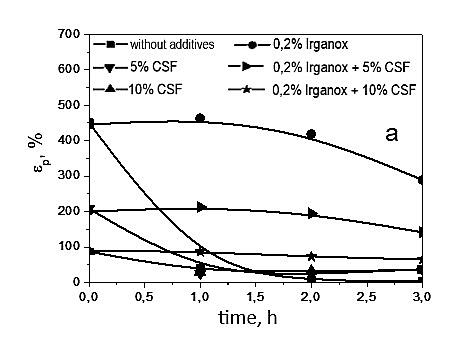
\includegraphics[width=\textwidth]{media/chem/image24}
    \end{subfigure}
    \hspace{0.05\textwidth} % Adjust horizontal space between the subfigures
    \begin{subfigure}[t]{0.4\textwidth} % Align at the top
        \centering
        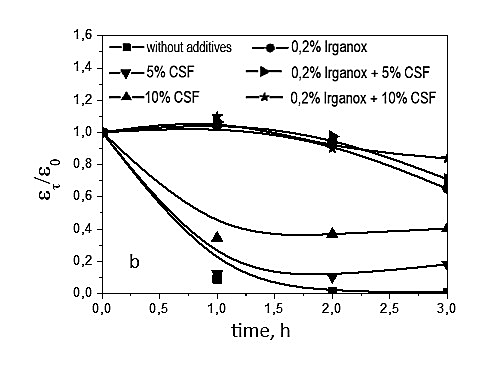
\includegraphics[width=\textwidth]{media/chem/image25}
    \end{subfigure}
    \caption*{Fig. 4 -- Change of yield strength (a) and breaking stress (b)
of composites in the process of thermal aging}
\end{figure}

\begin{multicols}{2}
{\bfseries Conclusions.} Thus, the studies that were conducted~have shown
that the use of CSF as a filler has a positive effect on the process of
thermal oxidation of high-pressure polyethylene, reducing its intensity.
The introduction of CSF into LDPE allows the yield strength after
the~exposition of samples for 3 hours at 170ºС at the level of 77\%
(10\% wt. CSF) and 46\% (5\% wt. CSF), while the ϭt of unfilled aged
LDPE does not exceed 3\% of the initial sample. The breaking stress of
the filled samples remains at the level of the unoxidized ones. The use
of this carbon-silicon filler in polyethylene compositions in
combination with a standard stabilizer makes it possible to practically
stop the~thermal aging of the polymer, thus extending its service life.
In spite of the fact that the introduction of 10\% wt. of CSF into the
polyethylene composition is more effective from the point of view of
ensuring thermal stability, it seems reasonable to use smaller amounts
of the filler. This is due to its negative effect on the elasticity of
the material since the introduction of 10\% wt. of CSF reduces the
relative elongation of the composition by 4.5 times compared to unfilled
LDPE. Nevertheless, the use of inexpensive filler from renewable plant
raw materials is of undoubted interest, because, being a product of
processing of agricultural waste, it allows to reduce the environmental
load and reduce the cost of polymer compositions.

\emph{{\bfseries Funding:} The work was carried out under the program of
targeted funding of scientific research for 2023-2025 IRN №BR21882289,
carried out by the Committee of Science of the Ministry of Science and
Higher Education of the Republic of Kazakhstan.}
\end{multicols}

\begin{center}
{\bfseries References}
\end{center}

\begin{references}
1.Popova L.A., Prokopchuk N.R., Yacenko V.V. Vliyanie napolnitelej na
stabilizacionnuyu ustojchivost'{} kompozicij polietilena
// Trudy BGTU. Seriya 4. Himiya i tekhnologiya organicheskih veshchestv
- 2009. - № 4. - S. 109-112. (In Russian).

2.Manulenko A.F., Lenartovich L.A., Prokopchuk N.R. Vliyanie
superkoncentratov napolnitelej i \\stabilizatorov na
termostabil' nost'{} polietilena // Trudy
BGTU. Seriya 2: Himicheskie tekhnologii,\\ biotekhnologiya, geoekologiya.
- 2016. - № 4(186). - S. 106-113. (In Russian)

3.Afashagova Z.H., Ovcharenko E.N., Kozlov G.V., Mikitaev A.K.
Termicheskie svojstva dispersno-napolnennogo polimernogo nanokompozita
// Izvestiya vuzov. Severo-Kavkazskij region. Seriya:\\ Estestvennye
nauki. 2007. №5.- S.34-36. (In Russian)

4.Lenartovich L.A., Prokopchuk N.R., SHkodich V.F. Teplovoe starenie
napolnennyh stabilizirovannyh kompozicij (obzor) //Vestnik
Tekhnologicheskogo universiteta. -2015. -T. 18.- № 9. -S. 41-48. (In
Russian)

5.Evrazijskij patent 045499 V1, MPK C08K 3/013, C08K 3/04, C08K 3/34.
Primenenie \\uglerod-kremnistogo kompozita v kachestve napolnitelya,
zayavl. 30.06.2021, opubl. 29.11. 2023. (In Russian)

6.Bobrova V.V., Prokopchuk N.R., Efremov S.A., Nechipurenko S.V.
Uglerod-kremnistyj napolnitel'{} dlya elastomernyh
kompozicij // Trudy BGTU. Seriya 2: Himicheskie tekhnologii,
biotekhnologiya, geoekologiya. - 2022. - № 1 (253). - S. 89-95. (In
Russian)

7.Song Y., Zeng L., Zheng Q. Understanding the reinforcement and
dissipation of natural rubber compounds filled with hybrid filler
composed of carbon black and silica // Chinese Journal of Polymer
Science. - 2017 -V. 35 - № 11. - P. 1436--1446. DOI
10.1007/s10118-017-1987-5

8.Xiong X., Wang J., Jia H., Ding L., Dai X., Fei X. Synergistic Effect
of Carbon Black and Carbon--Silica Dual Phase Filler in Natural Rubber
Matrix // Polymer Composites. - 2014.- V. 35 - № 8. - P. 1466--1472.
https://doi.org/10.1002/pc.22800

9.Sattayanurak S., Sahakaro K., Kaewsakul W., Dierkes W. K., Reuvekamp
L.A.E.M., Blume A., \\Noordermeer J.W.M. Synergistic effect by high
specific surface area carbon black as secondary filler in silica
reinforced natural rubber tire tread compounds // Polymer Testing --
2020-V.21-APP. 106173. DOI 10.1016/j.polymertesting.2019.106173

10.Velga V.D., Rossignol T.M., Crespo J. da S., Carli L.N. Tire tread
compounds with reduced rolling resistance and improved wet grip
//Journal of Applied Polymer Science. - 2017. - V.134- № 3 -- APP.
45334. DOI 10.1002/app.45334

11.Bobrova V.V., Prokopchuk N.R., Efremov S.A., Nechipurenko S.V.,
Stoyanov O.V. Vliyanie uglerod-kremnistogo napolnitelya na svojstva
elastomernyh kompozicij // Vestnik Tekhnologicheskogo universiteta. -
2022. - T. 25. - №6. - S. 86-90.
\href{https://www.elibrary.ru/item.asp?id=48660622}{https://www.elibrary.ru}. (In Russian)

12.Bobrova V.V., Prokopchuk N.R., Efremov S.A., Nechipurenko S.V.
Svojstva elastomernyh kompozicij, napolnennyh uglerod-kremnistym
kompozitom // Trudy BGTU. Seriya 2: Himicheskie tekhnologii,
\\biotekhnologiya, geoekologiya. - 2022. - № 2 (259). - S. 156-164.DOI
10.52065/2520-2669-2022-259-2-156-164 (In Russian)

13.Bobrova V.V., Prokopchuk N.R., Efremov S.A., Nechipurenko S.V.,
Stoyanov O.V. Elastomernye kompozicii, napolnennye produktom pererabotki
risa // Vestnik Tekhnologicheskogo universiteta. - 2023. - T. 26. - № 2.
- S. 60-63. \href{https://elib.belstu.by/handle/123456789/65005/}{https://elib.belstu.by} (In Russian).

14.Bobrova V.V., Prokopchuk N.R., Efremov S.A., Nechipurenko S.V.,
Stoyanov O.V. Vliyanie napolnitelya na osnove produktov pererabotki risa
na dolyu svyazannogo polimera v elastomernyh kompoziciyah // Vestnik
Tekhnologicheskogo universiteta. - 2023. - T. 26. - № 3. - S.
50-52.. \href{https://elib.belstu.by/handle/123456789/65006}{https://elib.belstu.by}. (In Russian)

15.Bobrova V.V., Prokopchuk N.R., Efremov S.A., Nechipurenko S.V.
Primenenie uglerod-kremnistogo napolnitelya v elastomernyh kompoziciyah
na osnove kombinacii kauchukov // Trudy BGTU. Seriya 2: Himicheskie
tekhnologii, biotekhnologiya, geoekologiya. - 2023. - № 1 (265). - S.
95-103. (In Russian).
\end{references}

\begin{authorinfo}
\hspace{1em}\emph{{\bfseries Information about authors}}

Vernigorov K.B.- General Manager SIBUR PolyLab LLC, Moscow, Russia,
e-mail:
\href{mailto:ov_stoyanov@mail.ru}{\nolinkurl{ov\_stoyanov@mail.ru}};

Nechipurenko S.V.- Candidate of Technical Sciences, Associate Professor,
Leading Researcher, Al-Farabi Kazakh National University, National
Engineering Academy of RK, Almaty, Kazakhstan, e-mail:
\href{mailto:nechipurenkos@mail.ru}{\nolinkurl{nechipurenkos@mail.ru}};

Yermukhambetova B.B. -Candidate of Chemical Sciences, Leading
Researcher, Al-Farabi Kazakh National University, National Engineering
Academy of RK, Almaty, Kazakhstan, e-mail:
\href{mailto:baya_yerm@mail.ru}{\nolinkurl{baya\_yerm@mail.ru}};

Bushkov V.V. - General Manager SIBUR LLC, Moscow, Russia, e-mail:
\href{mailto:ov_stoyanov@mail.ru}{\nolinkurl{ov\_stoyanov@mail.ru}};

Irmukhametova G.S. - Candidate of Chemical Sciences, Associate
Professor, Leading Researcher, Al-Farabi Kazakh National University,
National Engineering Academy of RK, Almaty, Kazakhstan, e-mail:
\href{mailto:galiya.irm@gmail.com}{\nolinkurl{galiya.irm@gmail.com}};

Alikulov A.Zh. - Master of Technical Sciences, Senior Lecturer,
Researcher, Al-Farabi Kazakh National University, National Engineering
Academy of RK, Almaty, Kazakhstan, e-mail:
\href{mailto:alikulov.adilet@gmail.com}{\nolinkurl{alikulov.adilet@gmail.com}};

Stoyanov O.V.- PhD, Professor, Kazan National Research Technological
University, Kazan, Russia, e-mail:
\href{mailto:ov_stoyanov@mail.ru}{\nolinkurl{ov\_stoyanov@mail.ru}};

Kazakov Y.M. - Doctor of Technical Sciences, Professor, Kazan National
Research Technological University, Kazan, Russia, e-mail:
\href{mailto:ov_stoyanov@mail.ru}{\nolinkurl{ov\_stoyanov@mail.ru}};

Efremov S.A. -- Doctor of Chemical Sciences, Professor, Chief
Researcher, Al-Farabi Kazakh National University, Academician of
KazNANS, National Engineering Academy of RK, Almaty, Kazakhstan, e-mail:
\href{mailto:efremsa@mail.ru}{\nolinkurl{efremsa@mail.ru}}

\hspace{1em}\emph{{\bfseries Информация об авторах}}

Вернигоров К.Б.-генеральный директор ООО «СИБУР ПолиЛаб», Москва,
Россия, e-mail:
\href{mailto:ov_stoyanov@mail.ru}{\nolinkurl{ov\_stoyanov@mail.ru}};

Нечипуренко С.В.-кандидат технических наук, ассоциированный профессор,
ведущий научный сотрудник, Казахский национальный университет им.
аль-Фараби, Национальная инженерная академия РК, Алматы, Казахстан,
e-mail:
\\\href{mailto:nechipurenkos@mail.ru}{\nolinkurl{nechipurenkos@mail.ru}};

Ермухамбетова Б.Б.-кандидат химических наук, ведущий научный сотрудник,
Казахский национальный университет им. аль-Фараби, Национальная
инженерная академия РК, Алматы, Казахстан, e-mail:
\href{mailto:baya_yerm@mail.ru}{\nolinkurl{baya\_yerm@mail.ru}};

Бушков В.В.- генеральный директор ООО «СИБУР», Москва, Россия, e-mail:
\href{mailto:ov_stoyanov@mail.ru}{\nolinkurl{ov\_stoyanov@mail.ru}};

Ирмухаметова Г.С.- кандидат химических наук, ассоциированный профессор,
ведущий научный сотрудник, Казахский национальный университет им.
аль-Фараби, Национальная инженерная академия РК, Алматы, Казахстан,
e-mail:
\\\href{mailto:galiya.irm@gmail.com}{\nolinkurl{galiya.irm@gmail.com}};

Аликулов А.Ж.- магистр технических наук, старший преподаватель, научный
сотрудник, Казахский национальный университет им. аль-Фараби,
Национальная инженерная академия РК, Алматы, Казахстан, e-mail:
\href{mailto:alikulov.adilet@gmail.com}{\nolinkurl{alikulov.adilet@gmail.com}};

Стоянов О.В.- PhD, профессор, Казанский национальный исследовательский
технологический университет, Казань, Россия, e-mail:
\href{mailto:ov_stoyanov@mail.ru}{\nolinkurl{ov\_stoyanov@mail.ru}};

Казаков Ю.М.- доктор технических наук, профессор, Казанский национальный
исследовательский технологический университет, Казань, Россия, e-mail:
\href{mailto:ov_stoyanov@mail.ru}{\nolinkurl{ov\_stoyanov@mail.ru}};

Ефремов С.А. -- доктор химических наук, профессор, главный научный
сотрудник, Казахский национальный университет им. аль-Фараби,
Национальная инженерная академия РК, академик КазНАЕН, Алматы,
Казахстан, e-mail:
\\\href{mailto:efremsa@mail.ru}{\nolinkurl{efremsa@mail.ru}}
\end{authorinfo}
